\begin{definition}
	\textbf{Capacity of an $s-t$ path} in $G_f$ is the capacity of the minimum capacity edge on the path.
\end{definition}

Modification to Ford-Fullerson Algorithm: augment along path of high capacity. We will not pushing ourselves by looking for the path with highest capacity since that might take too much time. Instead, we develop a strategy to find a path with reasonable high capacity by introducing a threshold $\Delta$. As long as possible, we augment along path of capacity at least $\Delta$. When no such path available, set $\Delta = \Delta / 2$.
\subsection{The Range of Delta}
So what is the highest/first $\Delta$ to consider: the largest power of 2 $\le$ capacity of some edge of leaving the source. We only consider this $\Delta$ because if we make $\Delta$ twice as large as this, then you will find no edge from the source have such capacity and therefore you will find no augmenting path.

On the other hand the smallest/last $\Delta$ to consider is 1. It means we considering all paths.
\subsection{Algorithm}
How to find augmenting path in the residual graph with capacity $\ge \Delta$?

Suppose you have a path with capacity at least $\Delta$ in the $G_f$ as following. 
\begin{figure}[H]
	\centering
	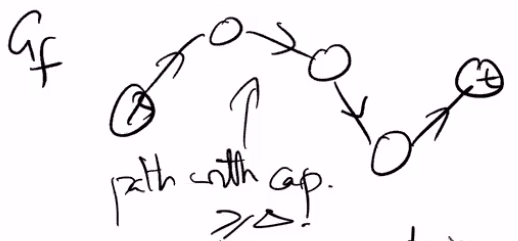
\includegraphics[width=0.5\textwidth]{fig/path-gf.png}
\end{figure}
Every edge on the path must has capacity $\ge \Delta$. Then we can define a subset of residual of graph called $G_f(\Delta)$, consisting only of edges with capacity $\ge \Delta$. Any path in $G_f(\Delta)$ from $s$ to $t$ will have capacity $\ge \Delta$.

Algorithm:
\begin{itemize}
	\item Start with 0 flow. Set $\Delta$ as described earlier. 
	\item Construct $G_f(\Delta)$.
	\item While there is an augmenting path in $G_f(\Delta)$, argument $f$ along this path. Reconstruct $G_f(\Delta)$ for the new flow and repeat.
	\item If there is no such path then set $\Delta = \Delta / 2$ and back to step 2 until $\Delta = 1$.
\end{itemize}

\subsection{Correctness}
\paragraph{Main Idea} Proof is same as the proof for Ford-Fulkerson's correctness. If you look at the new algorithm, it checks all the paths that Ford-Fulkerson uses. Even if it does not success finding the path when $\Delta$ has a high value, by the time $\Delta = 1$ you basically looking for all the augmenting paths. So you will find any the paths that exist.
\begin{definition}
	A phase of the algorithm is defined by a value of $\Delta$. So the number of phases is $O(\log C)$.
\end{definition}

How many augmentation can happen in each phase? 

When the $\Delta$-phase terminate we are ``pretty close'' to the optimal flow value. To quantify ``pretty close'', we make the following definition. 

\begin{definition}
	Let $f^*$ be the max flow. $|f^*|$ is the flow value of $f^*$. Let $f_{\Delta}$ be the flow at the end of the $\Delta$-phase. 
\end{definition}

\begin{theorem}
	$|f_{\Delta}| \ge |f^*| -m\Delta$, where $m$ is the number of edges in $G$.
\end{theorem}
\begin{proof}
	Consider the cut in $G_f(\Delta)$ at the end of the $\Delta$-phase, where $S$ consist of vertices reachable from $s$ in $G_f$ and $T$ consist of the others.
	\begin{figure}[H]
		\centering
		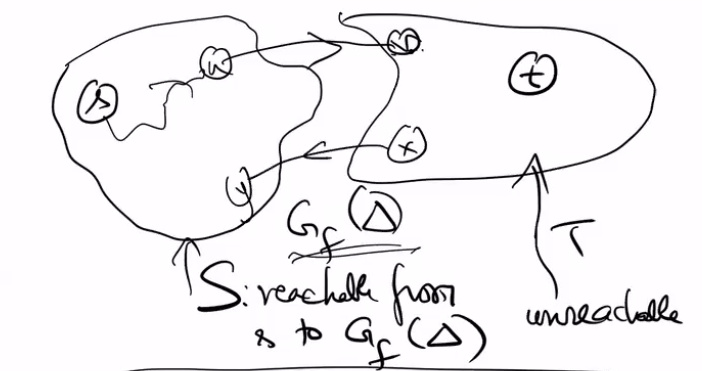
\includegraphics[width=0.6\textwidth]{fig/gf-delta.png}
	\end{figure}
	Look at this cut in the original graph $G$. Consider $u \in S$ and $v \in T$. If $(u, v)$ has residual capacity $\ge \Delta$. Then $(u, v)$ would have been present in $G_f(\Delta)$. This cannot happen because if $(u, v)$ has been present in $G_f(\Delta)$ then we are able to reach $u$ from $G_f(\Delta)$. If $(u, v)$ has residual capacity in $G_f(\Delta)$ then $v$ would be reachable as well. It is a contradiction because $v$ is actually not reachable from $S$ in $G_f(\Delta)$. .
	
	Therefore, $f(u,v) \ge c(u, v) - \Delta$. This is the only way that this edge would have residual capacity less than $\Delta$. 
	
	Now consider the edge $(x, y)$ in the back direction in the origin graph $G$, where $x \in T$ and $y \in S$. If $f(x, y) \ge \Delta$, then $(y, x)$ would have been present in $G_f(\Delta)$ with capacity $\ge \Delta$. It is also not possible since $x$ is not reachable. 
	
	Therefore, all backward edges carry at most flow $\Delta$.
	
	Based on the above facts, 
	\begin{align*}
		\text{net flow cross this cut} 
		\ge& \text{capacity of cut} - \Delta \times \text{(the number of edges across the cut)}\\
		\ge& \text{capacity of cut} - \Delta \times \text{(the number of edges in the graph)}
	\end{align*}
	
	Moreover, it is known that the capacity of cut is the upper bound of $|f^*|$. Therefore,
	
	\[|f_{\Delta}| \ge |f^*| - m\Delta\]	
\end{proof}
Based on the theorem, if we go to the next phase, $G_f(\frac{\Delta}{2})$, every augmentation increases the flow by at least $\frac{\Delta}{2}$. 

A phase starts with flow $f_{\Delta}$ can have at most $2m$ augmentation before flow value exceeds $|f^*|$. So for every phase, the number of augmentation is at most $2m$. Total number of augmentation across all phases $ = O(m \log C)$.


\subsection{Run Time Analysis}
How long does each augmentation take? 

We can construct $G_f(\Delta)$ in $O(m+n)$ time. DFS(or BFS) starting at $s$ will find an augmenting path to reach $t$ in $O(m+n)$ time if such a path exist. Overall running time is $O(m^2\log C)$.


